\section{Time-frequency map enhancement - skompilowac z Ferrara}\label{methodology_tf_enh}

In this section we present in details  the local maxima method which was previously based on non-overlapping windows in short time Fourier transform~\cite{Obuchowski2014325}. Here we describe how to adapt it to highly-overlapping windows.\\
The local maxima method starts with a transformation which converts a signal in time domain into a two-dimensional map (time-frequency), where spikes in time domain become wide-band excitations. In this paper we use the short-time Fourier transform that is denoted by $\{STFT(t,f)\}_{t\in T, f\in F}$, where $T$ is the set of time points and $F$ stands for the set of frequencies for which the transform is calculated. In the further analysis we assume $T=\{t_1,....,t_{\#T}\}$, where $\#T$ denotes number of elements of the set $T$. The STFT for random sample $X_1, ...,X_n$, time point $t_i$ and frequency $f$ is defined as follows:
\begin{eqnarray}
STFT(t_i,f)=\sum_{k=1}^{n}X_k\tilde{W}_{k-t_i}e^{jfk},
\end{eqnarray}
where $\{\tilde{W}_k\}$ is the window sequence.\\
Once the map is obtained, time series related to each $f\in F$ are analyzed.  For a given $f\in F$  and $t_i$ we put $M(t_i,f)=1$ if $|STFT(t_i,f)|=max\{|STFT(t_k,f)|: i-r\leq k\leq i+r\}$ and $M(t_i,f)=0$ elsewhere. The binary spectrogram obtained by applying this rule for every time series should have clearly visible wide-band excitations with small amount of local maxima between them if $r$ is properly chosen. We suggest  that $r$ (called the minimal neighborhood length) should be as high as it is possible to theoretically preserve all the cyclic wide-band excitations related to damage in a rotating machine. In the non-overlapping windows case $r$ is calculated as the highest integer value not greater than ratio of the expected time between the following disturbances to the STFT window length, both expressed in the same units, i.e. in samples or in a unit of time. The formula for $r$ is:
\begin{eqnarray}r=\left\lfloor (fs/ff)/Nw-1\right\rfloor\label{tf_enh_row1}
\end{eqnarray}
where $fs$ is the sampling frequency, $ff$ is the fault frequency, $Nw$ stands for the STFT window length and $\lfloor x\rfloor$ is the largest integer not greater than $x$. In the overlapping windows case we propose to modify equation (\ref{tf_enh_row1}) as follows:
\begin{eqnarray}\label{tf_enh_row2}
r=\left\lfloor ((fs/ff)/Nw-1)/(1-Ov)\right\rfloor,
\end{eqnarray}
where $Ov$ denotes overlap ratio, i.e. the ratio of the number of samples that each window overlaps to the window length. In the further analysis we use $Ov=0.95$ and compare it to $Ov=0$. In practice, there might be some deviations from the theoretical distance between local maxima. To illustrate this point, consider series of impulses of different height. It can be caused both by random character of shocks and random background noise. Relaxation of the impulses, even in local damage case, takes a little of time so the real distance between local maxima in a particular time series might be a little smaller than theoretical. Moreover, some of rotating machines exhibit jitter (e.g. bearings) during operation under constant rotational speed, so the real distance might be a little higher or lower than the distance obtained by using equation (\ref{tf_enh_row2}).\\
The next step in our procedure is to calculate the vector of weights and combine it with the binary spectrogram obtaining the enhanced spectrogram. The latter one is formulated as follows:
\begin{eqnarray}\label{tf_enh_row3}
ENH(t_i,f)=W(t_i)M(t_i,f),
\end{eqnarray}
where $W(t_i)=\frac{1}{\#F}\sum_{f\in F}M(t_i,f)$ is the vector of weights and $M(t_i,f)$  represents binary valued time series of the local maxima occurrence
for a time point  $t_i$ and frequency $f$. Conversion of the time-frequency map $\{|STFT(t,f)|\}_{t\in T, f\in F}$ into the binary matrix $\{M(t,f)\}_{t\in T, f\in F}$ preserves energy-invariance, i.e. local maxima in a low-energy frequency bin are as significant as local maxima in other frequency bin. An impulse in the vector of weights calculated as average value of $\{M(t_i,f)\}_{f\in F}$, for a particular time $t_i$ is present only if there is a significant number of local maxima at $t_i$, i.e. larger than in the case where local maxima at $t_i$ are the result of random character of the signal. If there are no wideband exciatations in the time-frequency map or frequency bands of the excitations are not significantly wide then the vector of weights has no pulses. Thus, in locally damaged machine case the enhanced time frequency map increases visibility of wideband excitations and decreases influence of high-energy components. In healthy machine case it presents time-frequency map without any pattern. Moreover, arithmetic mean in the formula for $W(t_i)$ makes the result invariant to number of points at which FFT is calculated.\\
In the next step of our procedure we propose to analyze the enhanced version of vector of weights, i.e. vector calculated as follows:
\begin{eqnarray}\label{tf_enh_row4}
V(t_i)=\frac{1}{\#F}\sum_{f\in F}ENH(t_i,f).
\label{tf_enh_enh_VoW}\end{eqnarray}
Formula~\ref{tf_enh_enh_VoW} reduces noise present in $\{W(t)\}_{t\in T}$ putting highes values to time points at which the enhanced spectrogram $\{ENH(t,f)\}_{t\in T, f\in F}$ has wideband excitations instead of taking into account only binary matrix $\{M(t,f)\}_{t\in T, f\in F}$ (as in $\{W(t)\}_{t\in T}$).\\
One of the tool useful to estimate the fault frequency is the sample autocorrelation function (ACF). For a random sample $Y_1,Y_2,...,Y_n$ the ACF  it is defined as follows:
\begin{eqnarray}
R(k)=\frac{\sum_{i=1}^{n-|k|}(Y_i-\bar{Y})(Y_{i+k}-\bar{Y})}{\sqrt{\sum_{i=1}^n(Y_i-\bar{Y})^2}},
\end{eqnarray}
where $\bar{Y}$ is a sample mean of the random sample $Y_1,Y_2,...,Y_n$. The vector of weights (and its enhanced version) is a set of non-negative real numbers including a set of significantly higher values in the case of local damage. If time intervals between these values are equal, then the sample ACF should be higher at lags related to them. It was shown that even in the case of poor resolution on time scale the sample ACF is sufficient to estimate the fault frequency.\\
The main purpose to use overlapping windows is better resolution on time scale. In this paper it will be examined whether the sample ACF will still be useful in the case of better time resolution. What is more, this examination will be preceded by analysis of envelope spectra in both overlapping and non-overlapping cases.\\
The whole procedure is presented in Fig.~\ref{tf_enh_fig01}
\begin{figure}[ht]
\begin{center}
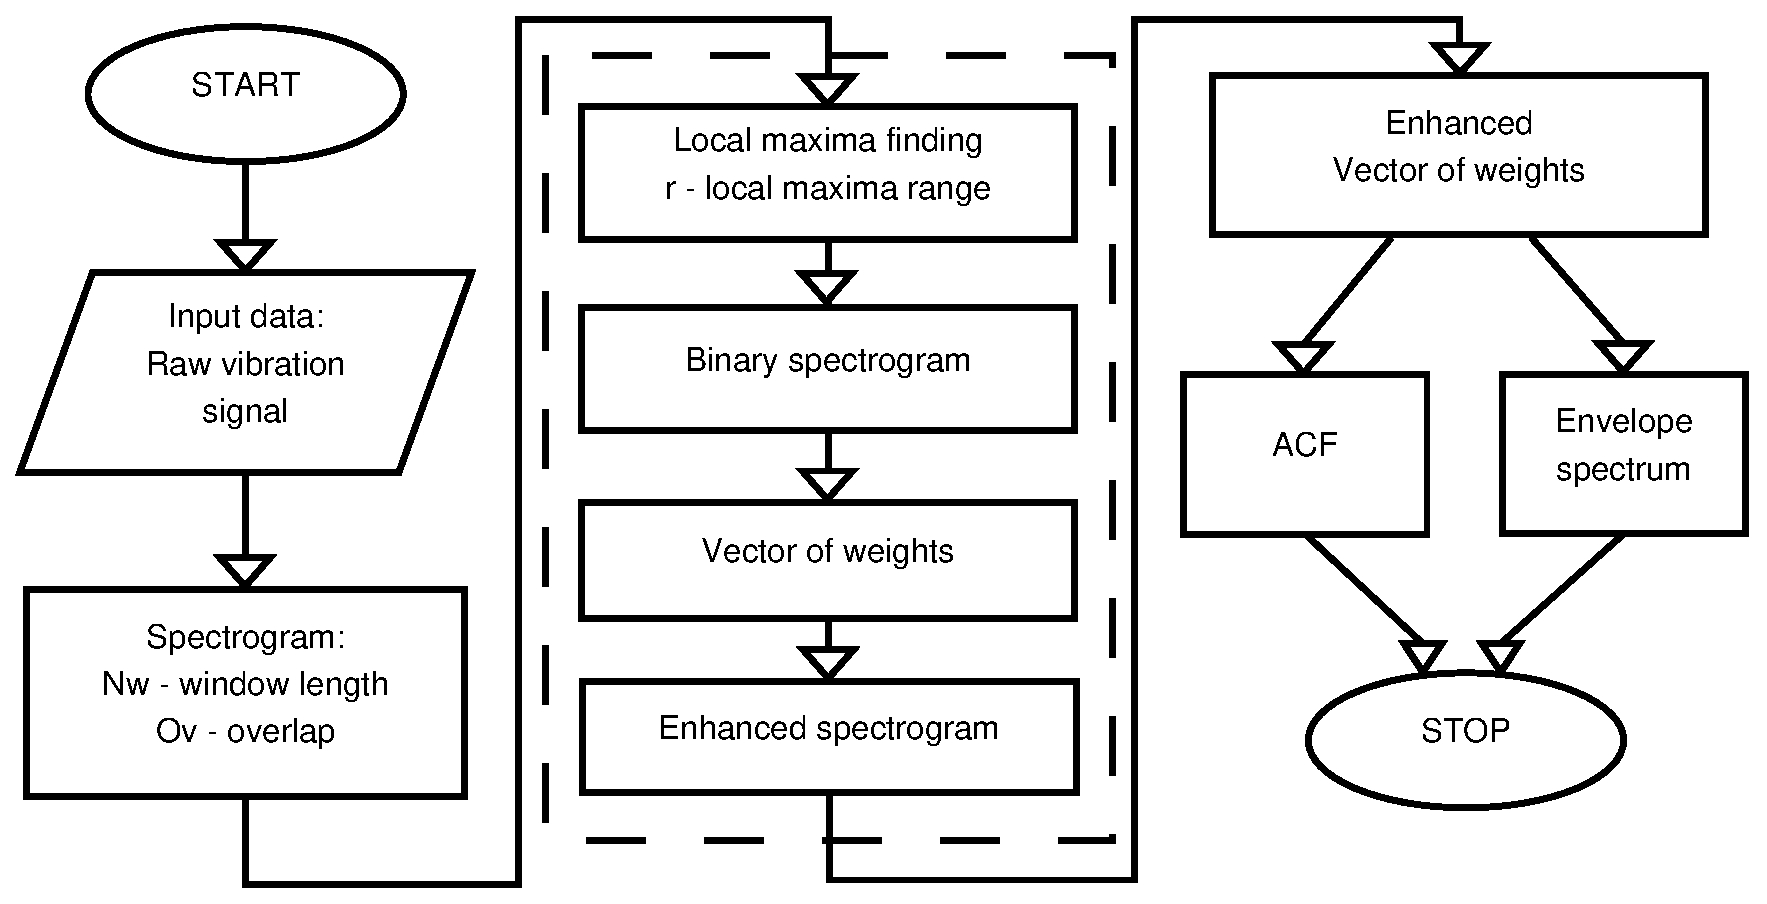
\includegraphics[width=0.7\textwidth]{methodology/tf_enh/fig01diagram}
\caption{Diagram of time-frequency map enhancement procedure.}\label{tf_enh_fig01}
\end{center}
\end{figure}
\FloatBarrier